\documentclass{beamer}
\usepackage[utf8]{inputenc}

\begin{document}

\title{Human-level control through \\ deep reinforcement learning}
\subtitle{A summary}
\author{David Prentiss}
\institute{OR750-004}
\date{\today}

\frame{\titlepage}

\begin{frame}
  \frametitle{Deep Q-network}
  \begin{itemize}
  \item Researchers set out to create a single algorithm that could learn a
    variety of tasks.
  \item Proposed Deep Q-network (DQN) model.
  \item Same model and hyperparameters trained on 49 different Atari 2600 games.
  \item Performance after training compared to human players and best linear learner.
  \item Adapted reinforcement learning methods to address stability issues
    with a non-linear approximator.
  \end{itemize}
\end{frame}

\begin{frame}
  \frametitle{Markov decision process}
  Markov decision process:
  \begin{itemize}
  \item discrete time steps, \(t\)
  \item set of states, \(S\)
  \item set of actions, \(A\)
  \item transition rule, \(P_a(s,s^\prime)=\text{Pr}(s_{t+1}=s^\prime\mid s_t=s, a_t=a)\)
  \item reward rule, \(R_a(s,s^\prime),\ R_a:S\times S \rightarrow \mathbb{R}\)
  \end{itemize}
\end{frame}

\begin{frame}
  \frametitle{Markov decision process}
  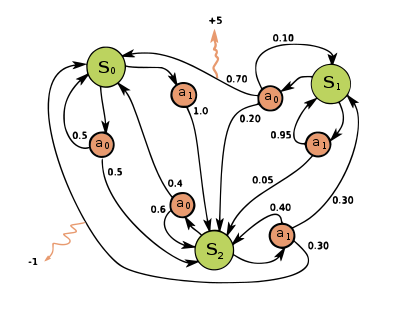
\includegraphics[width=\textwidth]{markov.png}
\end{frame}

\begin{frame}
  \frametitle{Markov decision process}
  \begin{itemize}
  \item Find the policy that maximizes expected reward over the process.
  \item \(\pi (a|s)=\text{Pr}(a_{t}=a|s_{t}=s)\)
  \item \(V_\pi(s)=\text{E}\left[
      \sum_{t=0}^\infty\gamma^tr_t\mid s_0=s
    \right]\)
  \item Can be solved with dynamic programming if all sets and rules are
    known.
  \end{itemize}
\end{frame}


\begin{frame}
  \frametitle{Reinforcement learning}
  \begin{itemize}
  \item Possibly unknown:
    \begin{itemize}
    \item set of states, \(S\)
    \item transition rule, \(P_a(s,s^\prime)=\text{Pr}(s_{t+1}=s^\prime\mid s_t=s, a_t=a)\)
    \item reward rule, \(R_a(s,s^\prime),\ R_a:S\times S \rightarrow \mathbb{R}\)
    \end{itemize}
  \item \(\pi (a|s)=\text{Pr}(a_{t}=a|s_{t}=s)\)
  \item The learning agent must ``explore'' to learn states and rewards.
  \item \(V^*(s)=\max_\pi V^\pi(s)\)
  \end{itemize}
\end{frame}

\begin{frame}
  \frametitle{Q-learning}
  \begin{itemize}
  \item Estimate action values rather than state values.
  \item Define \(Q:S\times A\rightarrow\mathbb{R}\)
    \begin{equation*}
      Q(s,a) = \text{E}
      \left[
        r_t + \gamma r_{t+1} + \gamma^2 r_{t+2}+\dots\mid s_t=s, a_t=a, \pi
      \right].
    \end{equation*}
  \item Represents the expected, future-discounted value of taking action
    \(a\) under state \(s\) and then following policy \(\pi\).
  \item Choosing action \(\text{argmax}_aQ^*(s_t,a)\) is equivalent to
    choosing \(\pi^*(s_t)\). (Due to Bellman's optimality principle?)
  \item Q-table update:
    \begin{equation*}
      Q^\prime(s_t,a_t) \leftarrow (1-\alpha)Q(s_t,a_t)+\alpha\left(r_t+\gamma\dot\max_aQ(S_{t+1},a)\right)
    \end{equation*}
  \end{itemize}
\end{frame}

\begin{frame}
  \frametitle{Q-learning}
  \begin{itemize}
  \item For large or continuous state sets it is necessary to approximate \(Q\).
  \item Nonlinear approximators may be desirable but may be unstable or
    divergent due to:
    \begin{itemize}
    \item Correlations in the sequence of observations
    \item Sensitivity of the policy to small changes in Q
    \item Correlations between action values \(Q\) and target values \(r+\gamma\max_{a^\prime}Q(s^\prime,a^\prime)\).
    \end{itemize}
  \item This work proposes to adapt a deep CNN as the Q approximator.
  \end{itemize}
\end{frame}

\begin{frame}
  \frametitle{DQN schematic}
  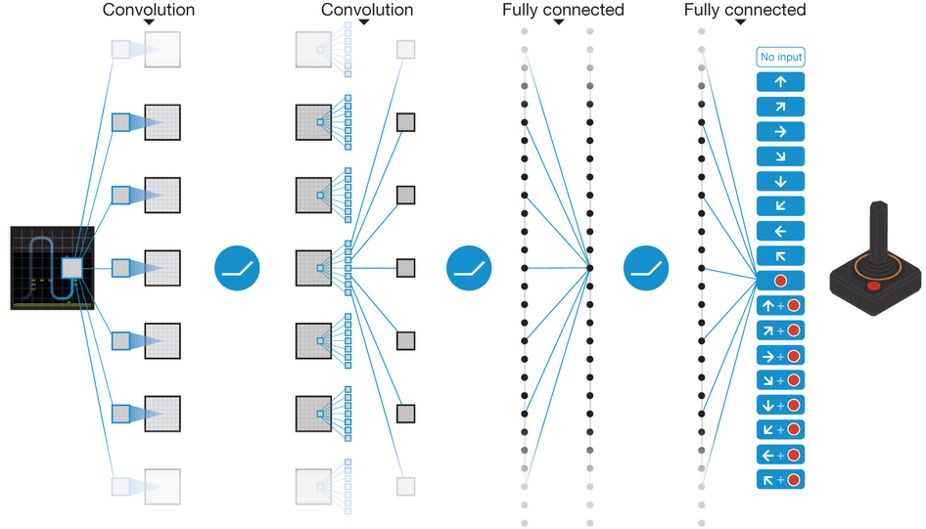
\includegraphics[width=\textwidth]{nature14236-f1.jpg}
\end{frame}

\begin{frame}
  \frametitle{DQN model features}
  \begin{itemize}
  \item The NN learns the optimal action-value function:
    \begin{equation*}
      Q^*(s,a) = \max_\pi\text{E}
      \left[
        r_t + \gamma r_{t+1} + \gamma^2 r_{t+2}+\dots\mid s_t=s, a_t=a, \pi
      \right].
    \end{equation*}
  \item Takes action from the policy with probability \(1-\epsilon\) or a random action with probability \(\epsilon\).
  \item Keeps a history, \(D\), of transitions \((\phi_t, a_t, r_t, \phi_{t+1})\).
  \item Trains on a uniformly sampled minibatch from of transitions from \(D\).
  \item Clones the network and use one copy for generating training targets and
    the other for training updates.
  \end{itemize}
\end{frame}

\begin{frame}
  \frametitle{Deep Q-learning with experience replay algorithm}
  Initialize sequence \(s_1=\{x_1\}\) and preprocessed sequence \(\phi=\phi(s_1)\) \\
  Initialize \(Q(\phi(s_t),a\mid\theta)\) and \(\hat{Q}(\phi(s_t),a\mid\theta^-)=Q\) \\
  \textbf{For} \(t=1, T\) \textbf{do}
  \\ \hspace*{20pt} With probability \(\epsilon\) select a random action \(a_t\)
  \\ \hspace*{40pt} or select \(a_t=\text{argmax}_a Q(\phi(s_t),a\mid\theta)\)
  \\ \hspace*{20pt} Execute action \(a_t\) in emulator
  \\ \hspace*{20pt} Observe reward \(r_t\) and image \(x_{t+1}\)
  \\ \hspace*{20pt} Store transition \((\phi_t, a_t, r_t, \phi_{t+1})\) in \(D\)
  \\ \hspace*{20pt} Sample minibatch of transitions \((\phi_j, a_j, r_j, \phi_{j+1})\) from \(D\)
  \\ \hspace*{20pt} Set \(y_j = r_j+\gamma\max_{a^\prime}\hat{Q}(\phi_{j+1},a^\prime\mid\theta^-)\)
  \\ \hspace*{20pt} Perform SGD step on \((y_j-Q(\phi_j,a_j\mid\theta))^2\)
  \\ \hspace*{20pt} Every \(C\) steps, reset \(\hat{Q}=Q\)

  \\ \textbf{End For}
\end{frame}

\begin{frame}
  \frametitle{Experience replay}
  \begin{itemize}
  \item Each step of experience is used many times for Q updates resulting in
    greater data efficiency.
  \item Correlations between consecutive samples is broken by training on a
    randomized sample of past experiences.
  \item This also breaks correlations between recent actions and the
    distribution of training data that might cause feedback loops.
  \item However, uniform sampling on a finite pool of past experiences
    is biased toward recent experiences.
  \item Gives equal weight to all transitions in the pool.
  \end{itemize}
\end{frame}

\begin{frame}
  \frametitle{Target generating network}
  \begin{itemize}
    \item DQN uses separate networks for generating targets \((\hat{Q})\) and updates \((Q)\).
      \item This also addresses the correlation between recent actions and
        training data distribution.
        \item Adds a delay between when an update is made and when that update
          effects the training targets.
  \end{itemize}
\end{frame}

\begin{frame}
  \frametitle{DQN performance}
  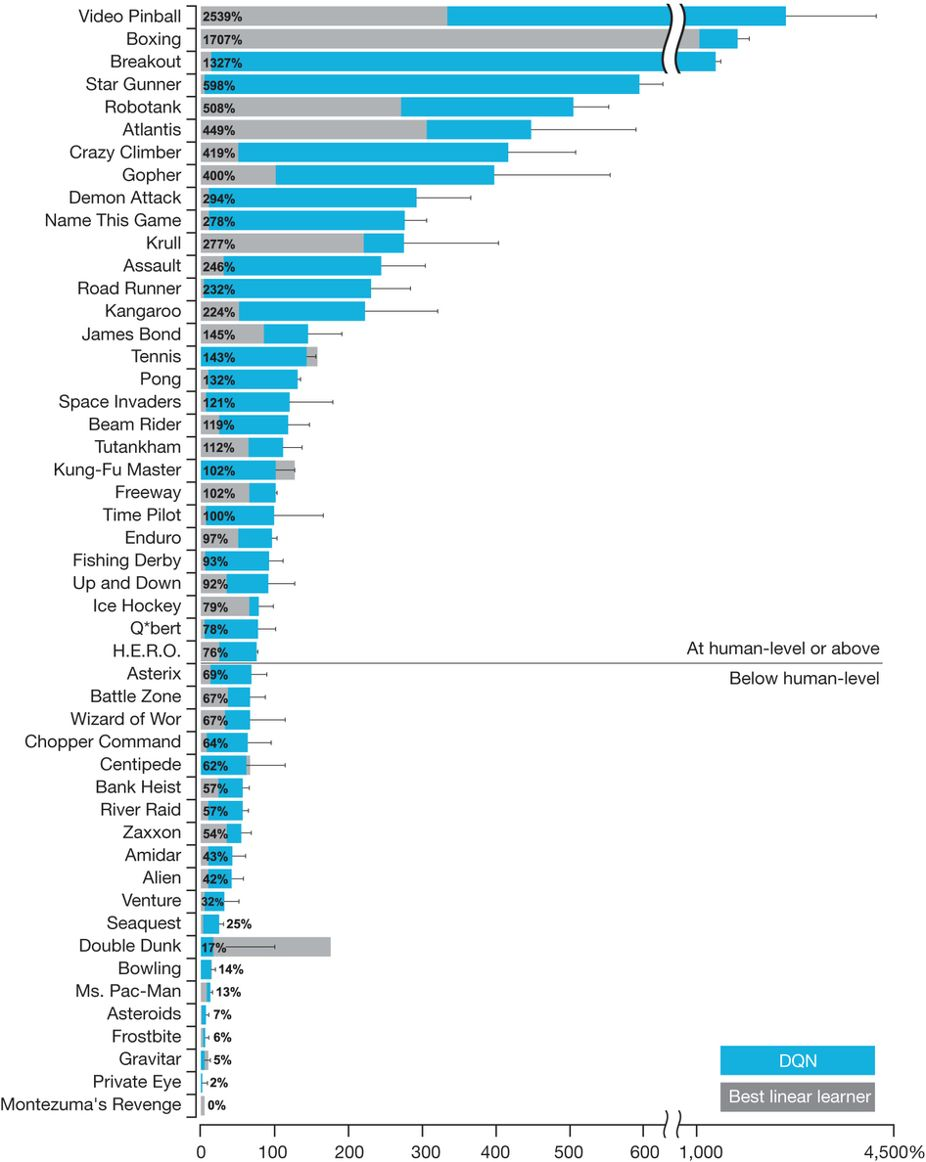
\includegraphics[width=\textwidth]{result.jpg}
\end{frame}

\end{document}